\chapter{Local Search}


With the spread of \emph{Model Driven Engineering} paradigms, more and more
tools appear to facilitate it. A common problem these tools face is the
efficient querying of graph patterns on the models. There are two main approach
to this problem with different benefits and drawbacks:

\begin{itemize}
  \item \emph{Local Search} - in this approach, the pattern matching is driven
  by a search plan, which contains simple checks and binding operations.
  \item \emph{Incremental Graph Matching} - this approach maintains a cache
  for the patterns based on the model while listening to any changes to the
  model and updating the caches as required.
\end{itemize}

For the problem of running graph matching algorithms in \emph{C++} over object
instances in an efficient manner, the local search based approach is easier to
implement, since it does not require notifications for object instance
lifecycle.

%----------------------------------------------------------------------------
\section{Pattern body graph}\label{sec:PatternBodyGraph}
%----------------------------------------------------------------------------

A \emph{pattern body graph} is a graphical representation of a graph pattern.
Figure \figref{patternBodyGraph} shows the pattern body graph of the previously
introduced pattern \emph{specializationCoursesOfTeacher}
(\listref{PatternCallIQPLExample}). On the pattern body graph, there are three
pattern variables, \emph{teacher}, \emph{course} and \emph{C}. The variable
teacher is constrained to be of Teacher type, while course is of Course type.
Variable C is an edge, and it's type is the courses association between Teachers
and Courses. The course variable is further constrained to be a
SpecializationCourse.

\begin{figure}[!ht]
\centering
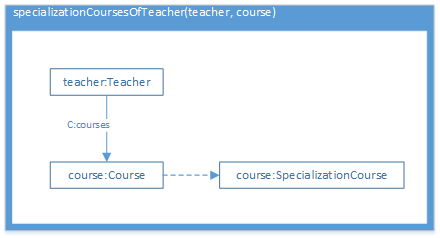
\includegraphics[width=110mm,
keepaspectratio]{figures/pattern_body_graph.png}
\caption{Pattern body graph of \emph{specializationCoursesOfTeacher}}
\label{fig:patternBodyGraph}
\end{figure}

%----------------------------------------------------------------------------
\section{Search graph}\label{sec:SearchGraph}
%----------------------------------------------------------------------------

The search graph is a graph based data structure of constraints and variables
for representing a query over a model. The search graph is a hypergraph, it's
edges represent constraints and nodes represent pattern variables. From the
original pattern graph, each node and edge turns into a pattern variable. The
constraints connect the constraints and arguments of the pattern graph, for
example if a constraint has a source and a target argument, the 3 nodes will be
connected with a source and a target edge.

This graph representation is very useful, since it allows for easy
simplification and normalization steps, which enhance the efficiency of the
query.

\begin{figure}[!ht]
\centering
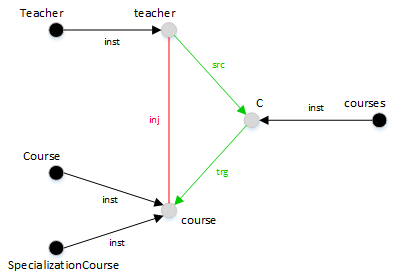
\includegraphics[width=110mm,
keepaspectratio]{figures/search_graph.png}
\caption{Search graph of \emph{specializationCoursesOfTeacher}}
\label{fig:searchGraph}
\end{figure}

Figure \figref{searchGraph} shows an example of the search graph of the
\emph{specializationCoursesOfTeacher} pattern. The search graph has seven
pattern variables. Pattern variables \emph{teacher}, \emph{course} and \emph{C}
represent variables (denoted by grey dots), while \emph{Teacher},
\emph{Course}, \emph{SpecializationCourse} and \emph{courses} represent types
(denoted by black dots). Between pattern variables and types, there are
\emph{``instance of''} constraints (black edges marked by \emph{inst}). Green
edges define the source and target of an edge (on the original pattern body
graph). Each node and each edge pattern variable from the pattern body graph
gets connected with an \emph{injectivity} constraint (red edge marked by \emph{inj}), meaning they
cannot be assigned the same value even if the other constraints would allow it.
Since there is only one edge pattern variable on the graph, there is no
injectivity constraint for it.

%----------------------------------------------------------------------------
\section{Search plan}\label{sec:SearchPlan}
%----------------------------------------------------------------------------

During the matching process, the search graph gets transformed into a search
plan. The transformation steps are shown on figure \figref{graph_to_plan}.

\begin{figure}[!ht]
\centering
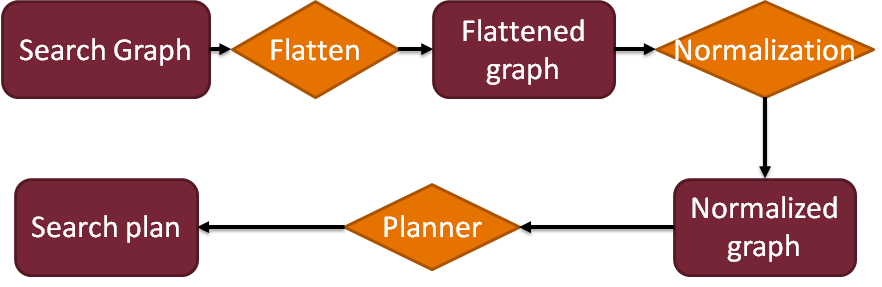
\includegraphics[width=130mm,
keepaspectratio]{figures/search_graph_plan_trans.png}
\caption{Search graph to search plan transformation}
\label{fig:graph_to_plan}
\end{figure}

The search graph may contain references to other queries. These references are
removed in the flattening step, where each reference is replaced with the
specified queries search graph. This results in the flattened search graph. The
next step is the normalization step. This removes any constraint deducable from
the metamodel, removes any duplicate or trivial constraints. The normalized
graph then gets sent to the planner which produces the search plan. 

The search plan is an ordered list of operations consisting of simple actions
applied to the model. The search graph have two basic types of operation:

\begin{itemize}
  \item extend - these operations assign a value to a variable based on a
  constraint. For example if a variable has a type constraint, then an object of
  the specified type will be bound to it.
  \item check - these kind of operations check whether the specified
  constraints are met on already bound variables, e.g. in case of a type
  constraint it checs if whether the object assigned to the variable is the
  specified type.
\end{itemize}

Executing the operations of the search plan in order while backtracking if an
operation fails results in objects assigned to the pattern variables which
satisfy the constraints.
